%%%%%%%%%%%%%%%%%%%%%%%%%%%%%%%%%%%%%%%%%%%%%%%
%%% Template for lab reports used at STIMA
%%%%%%%%%%%%%%%%%%%%%%%%%%%%%%%%%%%%%%%%%%%%%%%

%%%%%%%%%%%%%%%%%%%%%%%%%%%%%% Sets the document class for the document Openany
% is added to remove the book style of starting every new chapter on an odd page
% (not needed for reports)
\documentclass[11pt,english, openright, oneside]{book}

%%%%%%%%%%%%%%%%%%%%%%%%%%%%%% Loading packages that alter the style
\usepackage[]{graphicx}
\usepackage[]{color}
\usepackage{alltt}
\usepackage[T1]{fontenc}
\usepackage[utf8]{inputenc}
\usepackage{subcaption}
\usepackage{listings}
\usepackage{afterpage}
\usepackage{enumitem}
\newcommand\blankpage{%
    \null
    \thispagestyle{empty}%
    \newpage}

\usepackage[english, portuguese]{babel}

\usepackage[colorlinks = true, linkcolor = blue, urlcolor  = blue, citecolor =
            blue, anchorcolor = blue]{hyperref}

\newcommand{\MYhref}[3][blue]{\href{#2}{\color{#1}{#3}}}%

\renewcommand{\lstlistingname}{Anexos de Código}
\renewcommand{\lstlistlistingname}{Lista de \lstlistingname}

\setcounter{secnumdepth}{3}
\setcounter{tocdepth}{3}
\setlength{\parskip}{\smallskipamount}
\setlength{\parindent}{0pt}

\usepackage{listings}
\usepackage{color}

\definecolor{dkgreen}{rgb}{0,0.6,0}
\definecolor{gray}{rgb}{0.5,0.5,0.5}
\definecolor{mauve}{rgb}{0.58,0,0.82}
% Define some colors - Do professor
\definecolor{ListingColorKeyWord}{rgb}{0, 0.5, 0}
\definecolor{ListingColorComment}{rgb}{0.0, 0.0, 0.6}
\definecolor{ListingColorIdentifier}{rgb}{0.5, 0.12, 0.10}
\definecolor{ListingColorEmphasize}{rgb}{0, 1, 1}

\definecolor{ListingColorBreakLine}{rgb}{0.5, 0.12, 0.10}

\lstset{frame=tb, language=Java, aboveskip=3mm, belowskip=3mm,
  showstringspaces=false, columns=flexible, basicstyle={\small\ttfamily},
  numbers=none, numberstyle=\tiny\color{gray}, keywordstyle=\color{blue},
  commentstyle=\color{dkgreen}, stringstyle=\color{mauve}, breaklines=true,
  breakatwhitespace=true, tabsize=3 }

\lstset{ language=Python, keywordstyle={\color{ListingColorKeyWord}\bfseries},
	commentstyle=\color{ListingColorComment},
	identifierstyle=\color{ListingColorIdentifier}, basicstyle=\ttfamily,
	frame=single, showstringspaces=false, numbers=left, tabsize=2,
	breaklines=true,
	postbreak=\mbox{\textcolor{ListingColorBreakLine}{$\hookrightarrow$}}, }


\lstdefinelanguage{HTML5}{ language=html, sensitive=true, alsoletter={<>=-},
        otherkeywords={
        % HTML tags
        <html>, <head>, <title>, </title>, <meta, />, </head>, <body>, <canvas,
        \/canvas>, <script>, </script>, </body>, </html>, <!, html>, <style>,
        </style>, >< },  
        ndkeywords={
        % General
        =,
        % HTML attributes
        charset=, id=, width=, height=,
        % CSS properties
        border:, transform:, -moz-transform:, transition-duration:,
        transition-property:, transition-timing-function: },  
        morecomment=[s]{<!--}{-->}, tag=[s] }

\lstdefinelanguage{JavaScript}{ morekeywords={typeof, new, true, false, catch,
  function, return, null, catch, switch, var, if, in, while, do, else, case,
  break}, morecomment=[s]{/*}{*/}, morecomment=[l]//, morestring=[b]",
  morestring=[b]' }

% Set page margins
\usepackage[top=100pt,bottom=100pt,left=68pt,right=66pt]{geometry}

% Package used for placeholder text
\usepackage{lipsum}

% Prevents LaTeX from filling out a page to the bottom
\raggedbottom

% Adding both languages \usepackage[english, italian, portuguese]{babel}



\lstset{ language=python, %% Troque para PHP, C, Java, etc... bash é o padrão
    basicstyle=\ttfamily\small, numberstyle=\footnotesize, numbers=left,
    frame=single, tabsize=2, rulecolor=\color{black!30}, title=\lstname,
    escapeinside={\%*}{*)}, breaklines=true, breakatwhitespace=true,
    framextopmargin=2pt, framexbottommargin=2pt, inputencoding=utf8,
    extendedchars=true, literate={á}{{\'a}}1 {ã}{{\~a}}1 {é}{{\'e}}1
    {ç}{{\c{c}}}1, }


% All page numbers positioned at the bottom of the page
\usepackage{fancyhdr}
\fancyhf{} % clear all header and footers
\fancyfoot[C]{\thepage}
\renewcommand{\headrulewidth}{0pt} % remove the header rule
\pagestyle{fancy}
\renewcommand{\headrulewidth}{0.4pt}

% Changes the style of chapter headings
\usepackage{titlesec}
\titleformat{\chapter}
   {\normalfont\LARGE\bfseries}{\thechapter.}{1em}{}
% Change distance between chapter header and text
\titlespacing{\chapter}{0pt}{5pt}{2\baselineskip}

% Adds table captions above the table per default
\usepackage{float}
\floatstyle{plaintop}
\restylefloat{table}

% Adds space between caption and table
\usepackage[tableposition=top]{caption}

% Adds hyperlinks to references and ToC
\usepackage{hyperref}
\hypersetup{hidelinks,linkcolor = black} % Changes the link color to black and
% hides the hideous red border that usually is created

% If multiple images are to be added, a folder (path) with all the images can be
% added here 
\graphicspath{ {Figures/} }

% Separates the first part of the report/thesis in Roman numerals
\frontmatter

\usepackage[nottoc,numbib]{tocbibind}

\usepackage{listings}
\usepackage{color}

\usepackage{titlesec}
\titleformat{\chapter}[display]
  {\centering \normalsize \huge  \color{black}}{\thechapter}{10pt}{}



\definecolor{dkgreen}{rgb}{0,0.6,0}
\definecolor{gray}{rgb}{0.5,0.5,0.5}
\definecolor{mauve}{rgb}{0.58,0,0.82}

\lstset{frame=tb, language=Java, aboveskip=3mm, belowskip=3mm,
  showstringspaces=false, columns=flexible, basicstyle={\small\ttfamily},
  numbers=none, numberstyle=\tiny\color{gray}, keywordstyle=\color{blue},
  commentstyle=\color{dkgreen}, stringstyle=\color{mauve}, breaklines=true,
  breakatwhitespace=true, tabsize=3 }

%%%%%%%%%%%%%%%%%%%%%%%%%%%%%% Starts the document
\begin{document}

%%% Selects the language to be used for the first couple of pages
\selectlanguage{portuguese}


\renewcommand{\contentsname}{Índice}

%%%%% Adds the title page
\begin{titlepage}
	\clearpage\thispagestyle{empty}
	\centering
	\vspace{1cm}

	% Titles Information about the University
	{\Large \textbf{Redes de Internet}\par} {\Large Departamento de Engenharia
	Eletrónica e Telecomunicações e de Computadores \par} {\Large Instituto
	Superior de Engenharia de Lisboa \par}
		
	\vspace{0.5cm}
    
    \centering \includegraphics[scale=0.7]{imagens/ISEL.png}

	\vspace{1cm}
	
	{\Huge \textbf{Trabalho nº 3 (BGP for internet Configuration)}} \\
	\vspace{1cm}

        {\Large Licenciatura em Engenharia Informática e Multimédia}
        
	\vspace{0.5cm}
	
	
	
	
	\begin{center}
	{\normalsize Docente: \par Prof. Nuno Cruz \\
	
        \vspace{0.5cm}
              
        Alunos (Grupo 05):
        \par
        Alexandre Ferreira nº47485 
        \par 
        João Gonçalves nº47507
        \par
        Filipe Mendes nº48628
        
        \vspace{0.5cm} 
        Turma 52D
                
        \vspace{1cm}
        {\normalsize \today \par}
	             
	             
	             
	             \par}
	\end{center}
		
	% Set the date
	
	
	\pagebreak

\end{titlepage}

\tableofcontents
% Adds a table of contents
\pagebreak
\newpage


% Adds list of figures
\begingroup
\let\clearpage\relax
\pagebreak
\listoffigures
\endgroup

\newpage

% Adds list of tables
\begingroup
\let\clearpage\relax
\pagebreak
\listoftables
\endgroup

\newpage

\mainmatter
\chapter{Introdução}
\vspace{0.2cm}

\par Este relatório científico, elaborado no âmbito da unidade curricular de Redes de Internet, tem como objetivo explorar e aprofundar o conhecimento sobre a implementação do protocolo BGP (Border Gateway Protocol) em redes de computadores, com especial destaque na configuração de BGP entre diferentes Sistemas Autónomos (AS), representando Provedores de Serviços de Internet (ISP). O trabalho consiste na construção e configuração de uma topologia que simula a comunicação entre múltiplos AS, utilizando o BGP como protocolo de gateway externo (EGP) para estabelecer o encaminhamento de pacotes entre esses sistemas.
\vspace{0.2cm}

\par Ao longo do trabalho, foram realizadas diversas tarefas que incluíram a configuração do BGP para a troca de informações de encaminhamento entre os AS, a implementação de políticas de encaminhamento, e a verificação da conectividade entre os dispositivos da rede. Estas atividades permitiram observar o comportamento do protocolo BGP em diferentes cenários e testar a flexibilidade das suas políticas, bem como a escalabilidade e segurança do encaminhamento em ambientes simulados de internet. O relatório descreve em detalhe as configurações efetuadas, as justificações para cada escolha realizada, e os resultados obtidos, oferecendo uma visão abrangente das práticas de configuração e gestão aplicadas na operação de redes de computadores, utilizando o BGP.
\vspace{0.2cm}

\par A topologia de rede implementada é a seguinte imagem:
\vspace{0.2cm}

\begin{figure}[H]
  \centering
  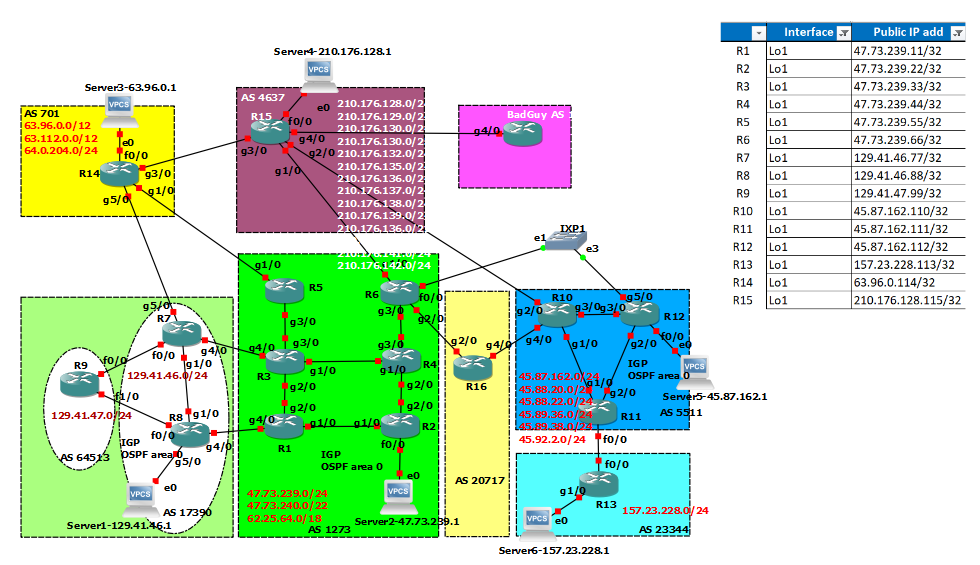
\includegraphics[width=0.73\textwidth]{imagens/topologia.png}
  \caption{Topologia de rede}
  \label{fig:topologia}
\end{figure}

\pagebreak

\chapter{Enquadramento Teórico}
\vspace{0.2cm}

Sendo que ao longo do documento são abordados o RIPv2, OSPF e BGP, abaixo sumarizar-se-ão os temas 
sob a forma de um glossário de modo a facilitar a compreensão dos tópicos: 

\begin{itemize}
  \item \textbf{OSPF}
  \vspace{0.2cm}
  \par O OSPF é um protocolo do tipo \textbf{link state}, de routing interno (\textbf{IGP - Internal Gateway Protocol}), dinâmico e "aberto", que pode ser implementado por qualquer fabricante sem o pagamento de licença, permitindo assim o seu uso generalizado. Apresenta diversas vantagens, como a inexistência de limites no número de saltos (hops), suporte ao encaminhamento \textbf{classless}, e \textbf{menor tráfego}, uma vez que as atualizações dos caminhos são enviadas com intervalos mais longos ou apenas quando ocorre uma alteração na topologia. Além disso, proporciona uma \textbf{convergência rápida}, \textbf{não cria loops}, reage prontamente às mudanças na rede, oferece um \textbf{melhor balanceamento} de carga, permite a \textbf{definição lógica de áreas}, facilitando a gestão da rede através do princípio de "dividir para reinar", possibilita a \textbf{marcação de rotas externas} e \textbf{suporta autenticação}.
  \vspace{0.2cm}

  Cada router \textbf{constrói um "mapa" da topologia da sua área}, trocando mensagens de \textbf{Link State Update} entre si para anunciar as ligações que possuem. Sempre que possível, utilizam \textbf{multicast} para essa comunicação. Cada router, então, calcula o \textbf{caminho mais curto} para todos os outros routers da área, utilizando o algoritmo de \textbf{Dijkstra}. A \textbf{tabela de routing} inclui a informação resultante deste cálculo, assim como a informação proveniente dos routers que fazem fronteira com outras áreas. Para manter a integridade da rede, os routers enviam constantemente mensagens \textbf{Hello} para verificar se os outros routers estão ativos. Caso um router não responda, os restantes routers da área são notificados e recalculam os melhores caminhos.
  \vspace{0.2cm}

  No contexto do OSPF, um grupo de routers que troca informações de encaminhamento entre si é denominado \textbf{Sistema Autónomo (AS)}. Este é constituído por um conjunto de redes que pode ser subdividido em várias \textbf{áreas} menores. A divisão em áreas traz vantagens, como ocultar a topologia de cada área das outras, isolar a eventual instabilidade de uma área das restantes e permitir que os routers necessitem de menos memória, dado que, sendo as áreas menores, o número de routers e redes em cada uma é reduzido, com as rotas para as outras \textbf{áreas a serem sumarizadas}.
  
  \newpage
  Adicionalmente, é importante mencionar os vários tipos de routers no OSPF:
  \begin{itemize}
    \item \textbf{Internal Router} em ligações apenas a routers da mesma área.
    \item \textbf{Area Border Router (ABR)} tem ligações a routers de outra área 0, sendo o responsável pela troca de informações de routing entre áreas. Cada ABR numa área sumariza para a área o custo para todas as redes externas à área. Depois de ser calculada a árvore SPF para a área, os caminhos para os destinos inter-área (exteriores à área) são calculados examinando os sumários dos ABR. 
    \item \textbf{Autonomous System Border Router (ASBR)} tem ligações a routers de outros Sistemas Autónomos. Também pode executar outros protocolos de routing (IGP ou EGP - RIP, EIGRP, BGP). 
    \item \textbf{Backbone Router} tem pelo menos uma interface que executa o OSPF na área 0.
  \end{itemize}
  \vspace{0.2cm}

  \item \textbf{BGP}
  \vspace{0.2cm}

  O Border Gateway Protocol (BGP) é um protocolo de routing, do tipo \textbf{path-vector}, utilizado para a troca de informações de encaminhamento entre Sistemas Autónomos (ASs).
  \vspace{0.2cm}

  No BGP:
  \begin{itemize}
    \item São anunciados caminhos completos, ou seja, uma lista de ASs.
    \item Os ciclos são detetados localmente e ignorados.
    \item As políticas locais permitem escolher o melhor caminho.
    \item Cada AS mantém uma tabela dos melhores caminhos.
    \item Quando uma ligação falha, o caminho é retirado.
  \end{itemize}
  \vspace{0.2cm}

  Alguns conceitos importantes de BGP:
  \begin{itemize}
    \item \textbf{Sessão BGP}: Ligação TCP entre dois peers BGP. Faz-se uso do keepalive para monitorizar o estado da sessão. 
    \item \textbf{Router fronteira}: Router com ligação a outras AS.
    \item \textbf{Tráfego de trânsito}: Tráfego que tem origem ou destino no AS em causa.
    \item \textbf{AS Path}: Lista de todos os AS atravessados por uma rota, no contexto da troa de informação 
    de encaminhamento.
    \item \textbf{Anúncio}: O BGP anuncia aos seus vizinhos todas as rotas para se alcançar um destino.
  \end{itemize}
  \vspace{0.2cm}

  \newpage
  Existem duas sessões BGP:
  \begin{itemize}
    \item \textbf{eBGP}: São sessões estabelecidas entres peers de AS diferentes.
    \item \textbf{iBGP}: São sessões estabelecidas entre peers do mesmo AS, tipicamente implementado com todos os peers interligados, também conhecido como full mesh. Quando se usa este método, há uma sobrecarga de processamento, havendo, por outro lado, métodos para minimizar a quantidade de ligações tal como:
    \begin{itemize}
      \item \textbf{Reflexão}: Apenas um peer iBGP é vizinho de todos os outros peer iBGP.
      \item \textbf{Confederações}: Divide-se um AS em vários sub-AS, utilizando números de AS privaddos, e apenas realizando o full mesh dentro dos sub-AS. 
    \end{itemize}
  \vspace{0.2cm}
  
  O BGP possui hierarquia, e 3 tipos de relações diferentes:
  \begin{itemize}
    \item \textbf{Fornecedor}: Anuncia todas as rotas aprendidas através de outros AS.
    \item \textbf{Cliente}: Anuncia todas as rotas que estão sobre o seu domínio e importa todas as rotas.
    \item \textbf{Peers}: Uma relação recíproca entre ISP que fornece conetividade a cada cliente de ambos.
  \end{itemize}
  \vspace{0.2cm}

  No protocolo BGP, existem 4 tipos de mensagem:
  \begin{itemize}
    \item \textbf{OPEN}: Abre uma ligação TCP para um peer e autentica o emissor.
    \item \textbf{UPDATE}: Anuncia novo caminho ou retira o antigo.
    \item \textbf{KEEPALIVE}: Mantêm a ligação aberta na ausência de mensagens de UPDATE, também serve como ACK ao pedido de OPEN.
    \item \textbf{NOTIFICATION}: Reporta erros nas mensagens anteriores ou fecha a ligação.
  \end{itemize}
  \vspace{0.2cm}

  Por fim, falta referir os atributos do BGP que permitem escolher a melhor rota, por exemplo. Alguns dos atributos mais recorrentemente falados são:
  \begin{itemize}
    \item \textbf{ORIGIN}: Indica como o BGP aprendeu sobre a rota particular (IGP, EGP ou Incomplete).
    \item \textbf{AS\_PATH}: Lista os números de AS que descrevem o percurso para atingir um destino.
    \item \textbf{NEXT\_HOP}: Endereço ip do router que se encontra no próximo salto para alcançar este destino.
    \item \textbf{MULTI\_EXIT\_DISC (MED)}: Quando um caminho inclui múltiplos ponto de saida ou entrada, este valor pode ser utilizado como métrica para escolher entre eles.
    \item \textbf{LOCAL\_PREF}: Utilizado entre BGP do mesmo AS para indicar o nível de preferência a um caminho de saída, em relação a um diferente.
    \item \textbf{WEIGHT}: Se um router aprende mais de uma rota para o mesmo destino, a rota com maio weight é a preferencial.
  \end{itemize}
\end{itemize}
\vspace{0.2cm}
\end{itemize}

É de notar que ao longo do desenvolvimento do projeto no \textbf{GNS3}, serão desenvolvidos ainda os conceitos estudados anteriormente.

\pagebreak

\chapter{Desenvolvimento}

\section{Tarefa 1 - CONFIGURE ALL THE IGP CONFIGS INTERNAL TO THE AS’S}
\vspace{0.2cm}

Nesta tarefa, será realizada a configuração dos protocolos internos de encaminhamento (IGP) dentro dos Sistemas Autónomos (AS) de acordo com o esquema de endereçamento fornecido e as regras de design definidas. O objetivo principal é configurar as interfaces de rede nos routers, aplicar o protocolo OSPF (Open Shortest Path First) para garantir uma comunicação eficiente entre os dispositivos dentro de cada AS e verificar a conectividade tanto dentro dos AS como entre diferentes AS’s. Para tal, serão configurados os endereços IP de cada interface, conforme a tabela de endereçamento fornecida.
\vspace{0.2cm}

Durante esta tarefa, também serão realizados testes para garantir que a infraestrutura privada dentro dos AS esteja corretamente configurada e que as interfaces estejam operacionais. A configuração do OSPF será verificada para assegurar que as relações de vizinhança estejam estabelecidas corretamente. Além disso, será realizada a validação de conectividade básica através de pings e do comando traceroute, para confirmar que o encaminhamento está a funcionar conforme o esperado, tanto internamente dentro do AS como entre os AS’s.
\vspace{0.2cm}

Após a configuração e verificação da conectividade, será importante salvar todas as configurações dos routers e do ambiente de simulação, garantindo que o progresso realizado seja guardado corretamente.

\vspace{0.2cm}

Foi fornecida a seguinte tabela (devido ao tamanho, foi dividia em 3):

\begin{table}[H]
\centering
\begin{tabular}{|c|c|c|c|}
\hline
\textbf{Router} & \textbf{Interface} & \textbf{Private IP Address} & \textbf{Public IP Address} \\ \hline
R1 & Loopback0 & 10.1.1.1 /32 & \\ \hline
R1 & Loopback1 & & 47.73.239.11 /32 \\ \hline
R1 & G1/0 & 10.1.2.1 /30 & \\ \hline
R1 & G2/0 & 10.1.3.1 /30 & \\ \hline
R1 & G4/0 &  & 47.73.240.1 /30 \\ \hline
R2 & Loopback0 & 10.2.2.2 /32 & \\ \hline
R2 & Loopback1 & & 47.73.239.22 /32 \\ \hline
R2 & f0/0 & & 47.73.239.2 /30 \\ \hline
R2 & G1/0 & 10.1.2.2 /30 & \\ \hline
R2 & G2/0 & 10.2.4.1 /30 & \\ \hline
R3 & Loopback0 & 10.3.3.3 /32 & \\ \hline
R3 & Loopback1 & & 47.73.239.33 /32  \\ \hline
R3 & G1/0 & 10.3.4.1 /30 & \\ \hline
R3 & G2/0 & 10.1.3.2 /30 & \\ \hline
R3 & G3/0 & 10.3.5.1 /30 & \\ \hline
R3 & G4/0 & & 47.73.240.5 /30 \\ \hline
R4 & Loopback0 & 10.4.4.4 /32 & \\ \hline
R4 & Loopback1 & & 47.73.239.44 /32 \\ \hline
R4 & G1/0 & 10.3.4.2 /30 & \\ \hline
R4 & G2/0 & 10.2.4.2 /30 & \\ \hline
R4 & G3/0 & 10.4.6.1 /30 & \\ \hline
R5 & Loopback0 & 10.5.5.5 /32 & \\ \hline
R5 & Loopback1 & & 47.73.239.55 /32 \\ \hline
R5 & G1/0 & & 63.112.0.2 /30 \\ \hline
R5 & G3/0 & 10.3.5.2 /30 & \\ \hline
R6 & Loopback0 & 10.6.6.6 /32 & \\ \hline
R6 & Loopback1 & & 47.73.239.66 /32 \\ \hline
R6 & f0/0 & & 47.73.240.17 /30 \\ \hline
R6 & G1/0 & & 47.73.240.13 /30 \\ \hline
R6 & G2/0 & & 47.73.240.21 /30\\ \hline
R6 & G3/0 & 10.4.6.2 /30& \\ \hline
R7 & Loopback0 & 10.7.7.7 /32 & \\ \hline
R7 & Loopback1 & & 129.41.46.77 /32 \\ \hline
R7 & f0/0 & & 129.41.46.9 /30 \\ \hline
R7 & G1/0 & 10.7.8.1 /30 & \\ \hline
R7 & G4/0 & & 47.73.240.6 /30 \\ \hline
R7 & G5/0 & & 63.112.0.6 /30 \\ \hline
\end{tabular}
\caption{Endereços IP}
\label{tab:ip1}
\end{table}

\begin{table}[H]
\centering
\begin{tabular}{|c|c|c|c|}
\hline
\textbf{Router} & \textbf{Interface} & \textbf{IP Address} & \textbf{Subnet Mask} \\ \hline
R8 & Loopback0 & 10.8.8.8 /32 & \\ \hline
R8 & Loopback1 & & 129.41.46.88 /32 \\ \hline
R8 & f0/0 & & 129.41.46.5 /30 \\ \hline
R8 & G1/0 & 10.7.8.2 /30 & \\ \hline
R8 & G4/0 & & 47.73.240.2 /30 \\ \hline
R8 & G5/0 & & 129.41.46.2 /30 \\ \hline
R9 & Loopback0 & 10.9.9.9 /32 & \\ \hline
R9 & Loopback1 & & 129.41.47.99 /32 \\ \hline
R9 & f0/0 & & 129.41.46.10 /30 \\ \hline
R9 & f1/0 & & 129.41.46.6 /30\\ \hline
R10 & Loopback0 & 10.10.10.10 /32 & \\ \hline
R10 & Loopback1 & & 45.87.162.110 /32 \\ \hline
R10 & G1/0 & 10.10.11.1 /30 & \\ \hline
R10 & G2/0 & & 210.176.129.2 /30 \\ \hline
R10 & G3/0 & 10.10.12.1 /30 & \\ \hline
R10 & G4/0 & & 45.88.20.1 /30 \\ \hline
R11 & Loopback0 & 10.11.11.11 /32 & \\ \hline
R11 & Loopback1 & & 45.87.162.111 /32 \\ \hline
R11 & f0/0 & & 45.88.20.5 /30 \\ \hline
R11 & G1/0 & 10.10.11.2 /30 & \\ \hline
R11 & G2/0 & 10.11.12.1 /30 & \\ \hline
R12 & Loopback0 & 10.12.12.12 /32 & \\ \hline
R12 & Loopback1 & & 45.87.162.112 /32 \\ \hline
R12 & f0/0 & & 45.87.162.2 /30 \\ \hline
R12 & G2/0 & 10.11.12.2 /30 & \\ \hline
R12 & G3/0 & 10.10.12.2 /30 & \\ \hline
R12 & G5/0 & & 47.73.240.18 /30 \\ \hline
R13 & Loopback0 & 10.13.13.13 /32 & \\ \hline
R13 & Loopback1 & & 157.23.228.113 /32 \\ \hline
R13 & f0/0 & & 45.88.20.6 /30 \\ \hline
R13 & G1/0 & & 157.23.228.2 /30 \\ \hline
R14 & Loopback0 & 10.14.14.14 /32 & \\ \hline
R14 & Loopback1 & & 63.96.0.114 /32 \\ \hline
R14 & f0/0 & & 63.96.0.2 /30 \\ \hline
R14 & G1/0 & & 63.112.0.1 /30 \\ \hline
R14 & G3/0 & & 63.112.0.9 /30 \\ \hline
R14 & G5/0 & & 63.112.0.5 /30 \\ \hline
\end{tabular}
\caption{Endereços IP}
\label{tab:ip1}
\end{table}


\begin{table}[H]
\centering
\begin{tabular}{|c|c|c|c|}
\hline
\textbf{Router / Equipment} & \textbf{Interface} & \textbf{Private IP Address} & \textbf{Public IP Address} \\ \hline
R15 & Loopback0 & 10.15.15.15 /32 & \\ \hline
R15 & Loopback1 & & 210.176.128.115 /32 \\ \hline
R15 & f0/0 & & 210.176.128.2 /30 \\ \hline
R15 & G1/0 & & 47.73.240.14 /30 \\ \hline
R15 & G2/0 & & 210.176.129.1 /30 \\ \hline
R15 & G3/0 & & 63.112.0.10 /30 \\ \hline
R15 & G4/0 &  & 210.176.129.5 /30 \\ \hline
R16 & Loopback0 & 10.16.16.16 /32 & \\ \hline
R16 & G2/0 & & 47.73.240.22 /30 \\ \hline
R16 & G4/0 & & 45.88.20.2 /30 \\ \hline
Badguy & Loopback0 & 10.66.66.66 /32 & \\ \hline
Badguy & G4/0 & & 210.176.129.6 /30 \\ \hline
Server1 & e0 & & 129.41.46.1 /30 \\ \hline
Server2 & e0 & & 47.73.239.1 /30 \\ \hline
Server3 & e0 & & 63.96.0.1 /30 \\ \hline
Server4 & e0 & & 210.176.128.1 /30 \\ \hline
Server5 & e0 & & 45.87.162.1 /30 \\ \hline
Server6 & e0 & & 157.23.228.1 /30 \\ \hline
\end{tabular}
\caption{Endereços IP}
\label{tab:ip1}
\end{table}
\vspace{0.2cm}

\newpage
\subsection{INTERFACE CONFIGURATION}
\vspace{0.2cm}

Para a configuração das interfaces de rede nos routers, foi necessário atribuir os endereços IP privados e públicos de acordo com a tabela de endereçamento fornecida. O OSPF também foi configurado para permitir a troca de informações de encaminhamento entre os routers dentro de cada AS. Para tal, foram necessários os seguintes comandos:
\vspace{0.2cm}

\begin{itemize}
  \item \textbf{interface}: Aceder ao modo de configuração de interface seguido da indentificação da interface a configurar.
  \item \textbf{ip address}: Atribuir o endereço IP privado (ou público) e a máscara de sub-rede à interface.
  \item \textbf{no shutdown}: Ativar a interface.
  \item \textbf{exit}: Sair do modo de configuração de interface.
  \item \textbf{write memory}: Salvar as configurações. 
  \item \textbf{router ospf 1}: Aceder ao modo de configuração OSPF, seguido da identificação do processo OSPF.
  \item \textbf{router id}: Atribuir o ID do router.
  \item \textbf{passive-interface}: Configurar a interface como passiva.
  \item \textbf{network point-to-point}: Configurar a interface como ponto-a-ponto.
  \item \textbf{network}: Seguido do endereço IP e máscara de sub-rede da interface a anunciar, bem como a área OSPF.
\end{itemize}
\vspace{0.2cm}

\newpage
Para os Routers, tal como se pode observar na figura \ref{fig:config1}, as configurações foram realizadas com sucesso no router 1.
\vspace{0.2cm}

\begin{figure}[H]
  \centering
  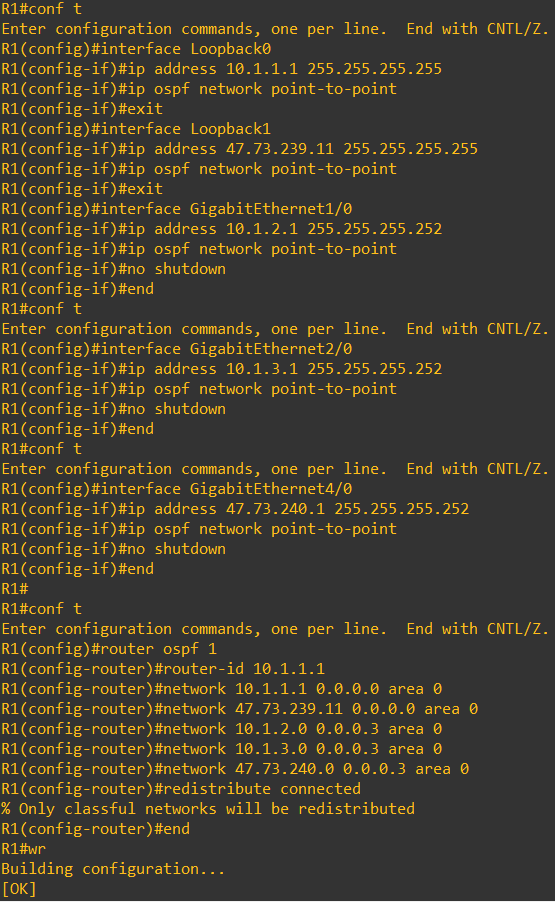
\includegraphics[width=0.70\textwidth]{imagens/Tarefa1/1.configR1.png}
  \caption{Configuração do Router 1}
  \label{fig:config1}
\end{figure}
\vspace{0.2cm}

\newpage
Para os Servers, tal como se pode observar na figura \ref{fig:configServer1}, as configurações foram realizadas com sucesso no Server 1.
\vspace{0.2cm}

\begin{figure}[H]
  \centering
  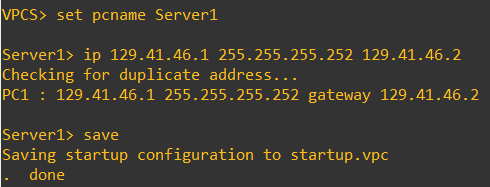
\includegraphics[width=0.70\textwidth]{imagens/Tarefa1/1.configServer1.png}
  \caption{Configuração do Server 1}
  \label{fig:configServer1}
\end{figure}
\vspace{0.2cm}

\subsection{VERIFY BASIC CONNECTIVITY}
\vspace{0.2cm}

Depois de configurar as interfaces de rede e o OSPF em cada router, é necessário verificar a conectividade básica entre os dispositivos dentro de cada AS.
\vspace{0.2cm}

Começando com teste de conectividade entre routers diretamente conectados, com o comando \textbf{ping}, foi possível confirmar que a comunicação entre os dispositivos está a funcionar corretamente. Tal como se pode observar na figura \ref{fig:testePing}, o ping foi bem sucedido entre o Router 1 para o Router 2 e o Router 13 para o 11.
\vspace{0.2cm}

\begin{figure}[h]
  \centering
  \begin{subfigure}{.5\textwidth}
      \centering
      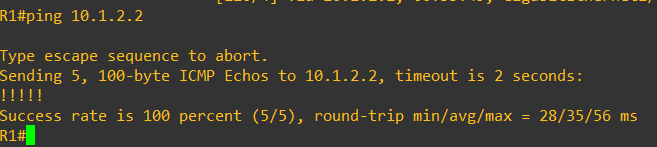
\includegraphics[width=0.99\linewidth]{imagens/Tarefa1/2.pingR1_R2.png}
  \end{subfigure}%
  \begin{subfigure}{.5\textwidth}
      \centering
      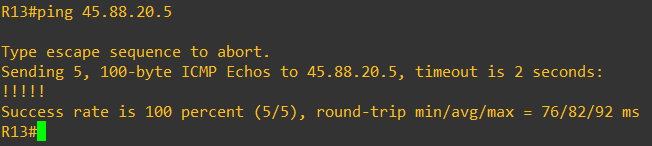
\includegraphics[width=0.99\linewidth]{imagens/Tarefa1/2.pingR13_R11.png}
  \end{subfigure}
  \caption{Teste de ping entre routers}
  \label{fig:testePing}
\end{figure}
\vspace{0.2cm}

\newpage
Também foi realizado um teste de conectividade entre routers não diretamente conectados, com o comando \textbf{traceroute}, para verificar o caminho percorrido pelos pacotes entre os dispositivos. Tal como se pode observar na figura \ref{fig:testeTraceroute}, o traceroute foi bem sucedido entre o Router 1 para o Router 2 e o Router 13 para o 11.
\vspace{0.2cm}

\begin{figure}[H]
  \centering
  \begin{subfigure}{.5\textwidth}
      \centering
      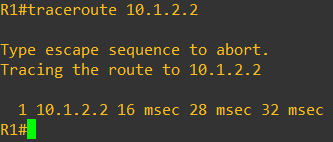
\includegraphics[width=0.94\linewidth]{imagens/Tarefa1/2.tracerouteR1_R2.png}
  \end{subfigure}%
  \begin{subfigure}{.5\textwidth}
      \centering
      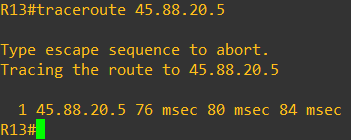
\includegraphics[width=1\linewidth]{imagens/Tarefa1/2.tracerouteR13_R11.png}
  \end{subfigure}
  \caption{Teste de traceroute entre routers}
  \label{fig:testeTraceroute}
\end{figure}
\vspace{0.2cm}

Vamos utilizar os comandos \textbf{show ip ospf neighbor} e \textbf{sh ip ospf interface brief} para verificar as relações de vizinhança OSPF e as interfaces OSPF, respetivamente. Tal como se pode observar na figura \ref{fig:showOspf}, as relações de vizinhança OSPF estão estabelecidas corretamente entre os routers e as interfaces OSPF estão ativas.
\vspace{0.2cm}

\begin{figure}[H]
  \centering
  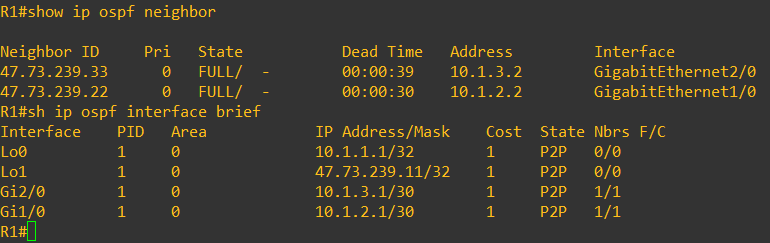
\includegraphics[width=0.70\textwidth]{imagens/Tarefa1/2.showOspf.png}
  \caption{Verificação de OSPF}
  \label{fig:showOspf}
\end{figure}
\vspace{0.2cm}

\newpage
Por fim, vamos utilizar o comando \textbf{ping} a todas as interfaces loopback dos routers para verificar a conectividade entre os dispositivos. Tal como se pode observar na figura \ref{fig:pingLoopback}, o ping foi bem sucedido entre os routers.
\vspace{0.2cm}

\begin{figure}[H]
  \centering
  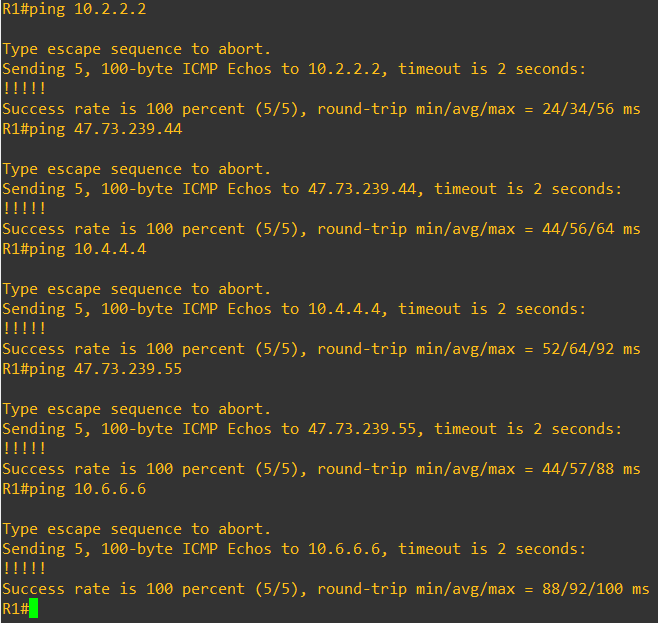
\includegraphics[width=0.70\textwidth]{imagens/Tarefa1/2.pingLoopback.png}
  \caption{Teste de ping entre loopbacks}
  \label{fig:pingLoopback}
\end{figure}
\vspace{0.2cm}

\subsection{REVIEW QUESTIONS}
\vspace{0.2cm}

\begin{enumerate}
  \item \textbf{What is the concept of an Autonomous System} 
  \vspace{0.2cm}

  Um Sistema Autónomo (AS) é um conjunto de redes e routers geridos por uma única entidade, que partilham uma política de encaminhamento comum utilizando um protocolo de routing associado a um único número de Sistema Autónomo (ASN). Os AS são fundamentais para a gestão e operação de redes de computadores, permitindo dividir a Internet em áreas mais facilmente geríveis e isoladas, cada uma com políticas de encaminhamento específicas.
  \vspace{0.2cm}

  \newpage
  \item \textbf{Use the https://bgp.tools/ and identify the AS’s entities involved in the lab topology.} 
  \vspace{0.2cm}

  Os Sistemas Autónomos (AS) visíveis na topologia são os seguintes:
  \vspace{0.2cm}

  \begin{itemize}
    \item \textbf{AS701 (Verizon Business)}: É um ISP Tier 1 global, ativo desde 1990, com 999 prefixos IPv4 e 38 IPv6, oferecendo conectividade sem depender de upstreams e participando em múltiplos IXPs.
    \item \textbf{AS4637 (Telstra Global)}: É um ISP global ativo desde 1995, com 572 prefixos IPv4 e 15 IPv6, alocado pela APNIC, oferecendo conectividade como operadora internacional.
    \item \textbf{BadGuy (1)}: É um AS suspeito, associado ao router marcado como "BadGuy".
    \item \textbf{AS64513}: É um ASN privado (Bogon ASN) com 3 prefixos IPv4 e nenhum IPv6, utilizado para redes internas ou testes, sem conectividade pública direta.
    \item \textbf{AS17390 (IBM)}: É um ASN ativo desde 2010, com 28 prefixos IPv4 e 21 IPv6, alocado pela ARIN, focado em redes corporativas e serviços "Eyeball" (acesso de utilizadores finais).
    \item \textbf{AS1273 (Vodafone Group PLC)}: É um ASN ativo desde 2002, com 177 prefixos IPv4 e 1 IPv6, alocado pela RIPE, operando como operadora internacional de telecomunicações.
    \item \textbf{AS20717 (DE-CIX Marseille Route Servers)}: É um ASN ativo desde 2015, alocado pela RIPE, sem prefixos próprios, usado para facilitar a troca de rotas entre redes através do ponto de troca de tráfego (IX) em Marselha.
    \item \textbf{AS5511 (Orange S.A.)}: É um ISP Tier 1 ativo desde 2002, alocado pela RIPE, com 314 prefixos IPv4 e 9 IPv6. A Orange oferece soluções de IP Transit e conectividade global, sendo um operador de telecomunicações de grande porte.
    \item \textbf{AS23344 (Disney Worldwide Services, Inc.)}: É um ASN ativo desde 2010, alocado pela ARIN, com 13 prefixos IPv4 e 13 IPv6. A Disney opera como uma rede de conteúdo, fornecendo serviços de distribuição de mídia e conteúdo através da Internet.
  \end{itemize}
  \vspace{0.2cm}

  \item \textbf{Identify tier 1 and tier 2 ISPs, explain the differences and the relations between them.} 
  \vspace{0.2cm}

  \begin{itemize}
    \item \textbf{Tier 1 ISP}:
    \vspace{0.2cm}

    \begin{itemize}
      \item \textbf{Exemplos na Topologia}: AS 701 (Verizon Business) e AS 4637 (Telstra Global).
      \item \textbf{Características}:
      \begin{itemize}
        \item Operadores globais com conectividade direta entre si.
        \item Não dependem de upstreams para alcançar qualquer destino na Internet.
        \item Realizam troca de tráfego (peering) gratuita com outros Tier 1 ISPs.
        \item Papel essencial na operação da Internet, assegurando conectividade global.
      \end{itemize}
    \end{itemize}
    \vspace{0.2cm}

    \newpage
    \item \textbf{Tier 2 ISP}:
    \vspace{0.2cm}
    \begin{itemize}
      \item \textbf{Exemplos na Topologia}: AS 1273 (Vodafone), AS 20717 (DE-CIX Marseille) e AS 5511 (Orange).
      \item \textbf{Características}:
      \begin{itemize}
        \item Operadores regionais ou nacionais que dependem de upstreams (geralmente ISPs Tier 1) para alcançar destinos fora da sua rede.
        \item Pagam pelo trânsito de dados para Tier 1 ISPs, mas podem também realizar peering com outros AS para reduzir custos e melhorar a eficiência.
      \end{itemize}
    \end{itemize}
    \vspace{0.2cm}
    \item \textbf{Relação entre Tier 1 e Tier 2 ISPs}:
    \vspace{0.2cm}
    \begin{itemize}
      \item Os Tier 2 ISPs dependem dos Tier 1 ISPs para conectividade global.
      \item \textbf{Exemplo na topologia:}:
      \begin{itemize}
        \item AS 1273 (Vodafone) utiliza AS 701 (Verizon Business) ou AS 4637 (Telstra Global) como upstream.
        \item AS 20717 (DE-CIX Marseille) estabelece peering com Tier 1 ISPs para melhorar a troca de rotas locais e regionais.
      \end{itemize}
    \end{itemize}
  \end{itemize}
  \vspace{0.2cm}


  \item \textbf{Identify in the topology, the peering’s between the AS’s.} 
  \vspace{0.2cm}

  Com base na topologia:
  \vspace{0.2cm}

  \begin{itemize}
    \item Entre AS 1273 (R1, R2, R3, R5, R6) e AS 20717 (R6):
    \begin{itemize}
      \item Peering estabelecido através de ligações diretas.
    \end{itemize}
    \item Entre AS 20717 (R6) e AS 4637 (R15):
    \begin{itemize}
      \item Conexão direta na interface GigabitEthernet.
    \end{itemize}
    \item Entre AS 20717 e AS 5511 (R10, R11, R12):
    \begin{itemize}
      \item Peering através do IX (IXP1).
    \end{itemize}
    \item Entre AS 5511 e AS 23344:
    \begin{itemize}
      \item Conexão através do IXP ou ligação direta.
    \end{itemize}
    \item O AS 1 (BadGuy) parece ligado ao AS 4637, possivelmente para injetar tráfego malicioso.
  \end{itemize}
  \vspace{0.2cm}
  \item \textbf{Identify the neutral public peering interconnections in this lab topology.} 
  \vspace{0.2cm}

  \begin{itemize}
    \item IXP1 (Internet Exchange Point) é o ponto de interligação público identificado na topologia.
    \item Permite a troca de tráfego entre os seguintes AS:
    \begin{itemize}
      \item AS 5511 (R10, R11, R12).
      \item AS 20717 (através de R6).
      \item Outros AS como AS 23344 podem também estar ligados.
    \end{itemize}
  \end{itemize}
\end{enumerate}
\pagebreak

\section{Tarefa 2 - BGP IMPLEMENTATION WITHOUT ANY POLICY OR ROUTING RESTRICTIONS}
\vspace{0.2cm}




\subsection{REVIEW QUESTIONS}
\vspace{0.2cm}

\begin{enumerate}
  \item \textbf{You applied the configuration next-hop-self on the iBGP peering explain why} 
  \vspace{0.2cm}

  A configuração \textbf{next-hop-self} é utilizada em sessões iBGP para garantir que os next-hops das rotas aprendidas entre vizinhos iBGP sejam sempre alcançáveis dentro do mesmo AS (Sistema Autónomo). Quando um router iBGP anuncia uma rota a um vizinho iBGP, ele substitui o próximo salto original pelo seu próprio endereço IP, geralmente associado à sua interface Loopback.

  Sem esta configuração, o próximo salto de uma rota seria o endereço IP do router que originalmente anunciou a rota (por exemplo, um router externo via eBGP), o que pode causar problemas de encaminhamento se este endereço não for alcançável dentro do AS. Com o \textbf{next-hop-self}, o router iBGP redefine o próximo salto para o seu próprio endereço IP, simplificando o encaminhamento interno e garantindo que os vizinhos iBGP consigam sempre encaminhar corretamente o tráfego para o próximo salto.
  \vspace{0.2cm}

  \item \textbf{How are the route prefixes propagated inside the AS when you have the route reflectors configured?} 
  \vspace{0.2cm}

  Com a configuração de route reflectors (RR), a propagação de prefixos dentro de um AS torna-se mais eficiente, eliminando a necessidade de uma malha total (full mesh) de sessões iBGP. Os routers iBGP são divididos em dois grupos: route reflectors (RRs) e route reflector clients (RRCs).

  Os clientes (RRCs) anunciam os seus prefixos aos route reflectors, que têm a responsabilidade de refletir essas rotas para os restantes clientes e também para outros route reflectors, caso existam. Isto assegura que todos os routers iBGP dentro do AS recebam as rotas, mesmo que não estejam diretamente ligados entre si.
  
  Desta forma, o uso de RRs reduz significativamente o número de sessões iBGP necessárias, melhorando a escalabilidade da rede e simplificando a configuração.
  \vspace{0.2cm}

  \item \textbf{How is the BGP next hop reachability solved inside an AS?} 
  \vspace{0.2cm}

  A alcançabilidade do next-hop em BGP dentro de um AS é resolvida através das rotas presentes na tabela de encaminhamento do IGP (como OSPF ou IS-IS). O IGP é responsável por anunciar as interfaces utilizadas como next-hop, geralmente os endereços IP das interfaces Loopback dos routers, para garantir que todos os routers dentro do AS possam alcançar esses endereços.

  Adicionalmente, em sessões iBGP, a configuração do comando next-hop-self pode ser utilizada para simplificar o encaminhamento. Com este comando, o router que anuncia uma rota a um vizinho iBGP substitui o next-hop original pelo seu próprio endereço IP (normalmente o da sua Loopback). Isto assegura que o próximo salto é sempre acessível dentro do AS, mesmo que o próximo salto original (por exemplo, de um router externo) não seja diretamente alcançável.

  Desta forma, a combinação de IGP e next-hop-self garante conectividade e simplifica a propagação de rotas dentro do AS.
  \vspace{0.2cm}

  \item \textbf{What is the behaviour from BGP when the prefix next-hop is not reachable} 
  \vspace{0.2cm}

  Quando o next-hop de um prefixo BGP não é alcançável, a rota é considerada inválida e não é instalada na tabela de encaminhamento BGP (Loc-RIB). Para que uma rota seja válida, o BGP exige que o next-hop esteja presente na tabela de roteamento subjacente, seja ela fornecida por um protocolo IGP (como OSPF ou IS-IS) ou por uma rota estática.

  Se o next-hop não for resolvido, o BGP não pode encaminhar o tráfego para esse destino, pois depende da conectividade IP subjacente para alcançar os next-hops anunciados. Como consequência, o prefixo é descartado e não é propagado nem utilizado no encaminhamento. Este comportamento garante que apenas rotas funcionalmente alcançáveis sejam consideradas para o tráfego na rede.

  \vspace{0.2cm}

  \item \textbf{Why is a good practice the loopback IP address utilization in the iBGP sessions?} 
  \vspace{0.2cm}

  A utilização de endereços IP Loopback em sessões iBGP é considerada uma boa prática devido às seguintes principais razões:

  \begin{itemize}
    \item \textbf{Alta Disponibilidade}: As interfaces Loopback são virtuais e não dependem de hardware físico específico, o que significa que permanecem ativas desde que o router esteja funcional. Isto evita que uma falha numa interface física afete a sessão BGP.
    \item \textbf{Conectividade Redundante}: Como os endereços de Loopback são anunciados no IGP (como OSPF ou IS-IS), podem ser alcançados através de múltiplos caminhos. Isto garante maior resiliência e permite que a conectividade entre os routers seja mantida mesmo em caso de falha de um enlace físico.
    \item \textbf{Estabilidade}: Os endereços de Loopback são estáticos e independentes de interfaces físicas, simplificando a configuração e reduzindo a probabilidade de alterações inesperadas devido a alterações de topologia.
    \item \textbf{Escalabilidade}: Permite estabelecer sessões iBGP entre routers em diferentes localizações sem depender de interfaces físicas diretas, o que facilita a expansão da rede.
    \item \textbf{Simplificação do Encaminhamento}: A utilização de endereços Loopback evita a necessidade de lidar com alterações dinâmicas em endereços IP associados a interfaces físicas, simplificando a configuração de políticas e tabelas de encaminhamento.
    \item \textbf{Compatibilidade com Redundância e Balanceamento de Carga}: Com múltiplos caminhos redundantes para as Loopbacks, a rede pode implementar balanceamento de carga, distribuindo o tráfego de forma mais eficiente.
  \end{itemize}
  \vspace{0.2cm}

  Em resumo, o uso de endereços Loopback oferece maior robustez, redundância e simplicidade na configuração e operação de redes BGP.
  \vspace{0.2cm}

  \item \textbf{Observe in the Wireshark and add to the report a trace from a BGP session establishment and described 
  the packets and respective relation with the following stats.} 
  \vspace{0.2cm}

  No protocolo BGP, a máquina de estados segue a seguinte sequência durante o estabelecimento de uma sessão:

  \begin{enumerate}
    \item \textbf{Idle}: 
    \begin{itemize}
      \item É o estado inicial. O router aguarda a configuração da sessão BGP.
      \item Neste estado, o BGP realiza verificações básicas, como validação do vizinho e recursos disponíveis.
      \item Se estiver tudo em ordem, tenta avançar para o próximo estado.
    \end{itemize}
    \item \textbf{Connect}: 
    \begin{itemize}
      \item O router tenta estabelecer uma conexão TCP com o vizinho BGP na porta 179.
      \item Se a conexão for bem-sucedida, avança para o estado OpenSent. Caso contrário, transita para o estado Active.
    \end{itemize}
    \item \textbf{Active}: 
    \begin{itemize}
      \item O router continua à espera de uma conexão TCP do vizinho BGP.
      \item Se a conexão for estabelecida, o estado muda para OpenSent. Caso contrário, pode retornar ao estado Connect ou permanecer no estado Active, dependendo do temporizador.
    \end{itemize}
    \item \textbf{OpenSent}:
    \begin{itemize}
      \item O router envia uma mensagem OPEN ao vizinho para iniciar a sessão BGP.
      \item Aguarda a mensagem OPEN de resposta do vizinho.
      \item Se a mensagem for válida, transita para o estado OpenConfirm.
    \end{itemize}
    \item \textbf{OpenConfirm}: 
    \begin{itemize}
      \item O router recebeu a mensagem OPEN do vizinho e aguarda uma mensagem de confirmação KEEPALIVE.
      \item Se a mensagem KEEPALIVE for recebida corretamente, o estado muda para Established.
      \item Caso haja um erro (por exemplo, parâmetros incompatíveis), o estado pode voltar para Idle.
    \end{itemize}
    \item \textbf{Established}:
    \begin{itemize}
      \item A sessão BGP está ativa e os dois routers iniciam a troca de mensagens UPDATE para partilhar informações de rota.
      \item Enquanto a sessão estiver no estado Established, o BGP mantém a conexão viva através de mensagens KEEPALIVE.
    \end{itemize}
  \end{enumerate}

  \vspace{0.2cm}
  Durante o estabelecimento de uma sessão BGP, os pacotes trocados podem ser identificados pelas seguintes etapas:

  \begin{enumerate}
    \item \textbf{TCP 3-Way Handshake}:
    \begin{itemize}
      \item Antes de o BGP iniciar, é necessário estabelecer uma conexão TCP entre os vizinhos BGP na porta 179.
      \item Esta conexão é feita através da troca dos seguintes pacotes:
      \begin{itemize}
        \item \textbf{SYN}: O router inicia a solicitação de conexão TCP.
        \item \textbf{SYN-ACK}: O vizinho confirma a solicitação de conexão.
        \item \textbf{ACK}: O router finaliza o handshake, estabelecendo a conexão TCP.
      \end{itemize}
    \end{itemize}
    \item \textbf{BGP OPEN Message}:
    \begin{itemize}
      \item Após o TCP handshake, os routers trocam mensagens OPEN para iniciar a sessão BGP.
      \item EEstas mensagens contêm parâmetros essenciais, como a versão do BGP, o número do sistema autónomo (AS), o identificador BGP e as opções de capacidades, como suporte para extensões.
    \end{itemize}
    \item \textbf{BGP KEEPALIVE Messages}:
    \begin{itemize}
      \item Após o envio da mensagem OPEN, os routers trocam mensagens KEEPALIVE para confirmar que a sessão foi estabelecida corretamente.
      \item EEstas mensagens são enviadas periodicamente para manter a sessão ativa e confirmar a conectividade entre os vizinhos.
    \end{itemize}
    \item \textbf{BGP UPDATE Messages}:
    \begin{itemize}
      \item Com a sessão estabelecida, os routers começam a enviar mensagens UPDATE.
      \item Estas mensagens são utilizadas para anunciar ou retirar prefixos de rotas, partilhando informações de encaminhamento.
    \end{itemize}
  \end{enumerate}
  \vspace{0.2cm}

  Tal como se pode observar na figura \ref{fig:wireshark}, o estabelecimento de uma sessão BGP envolve a troca de mensagens OPEN, KEEPALIVE e UPDATE, conforme descrito acima.
  \vspace{0.2cm}

  \begin{figure}[H]
    \centering
    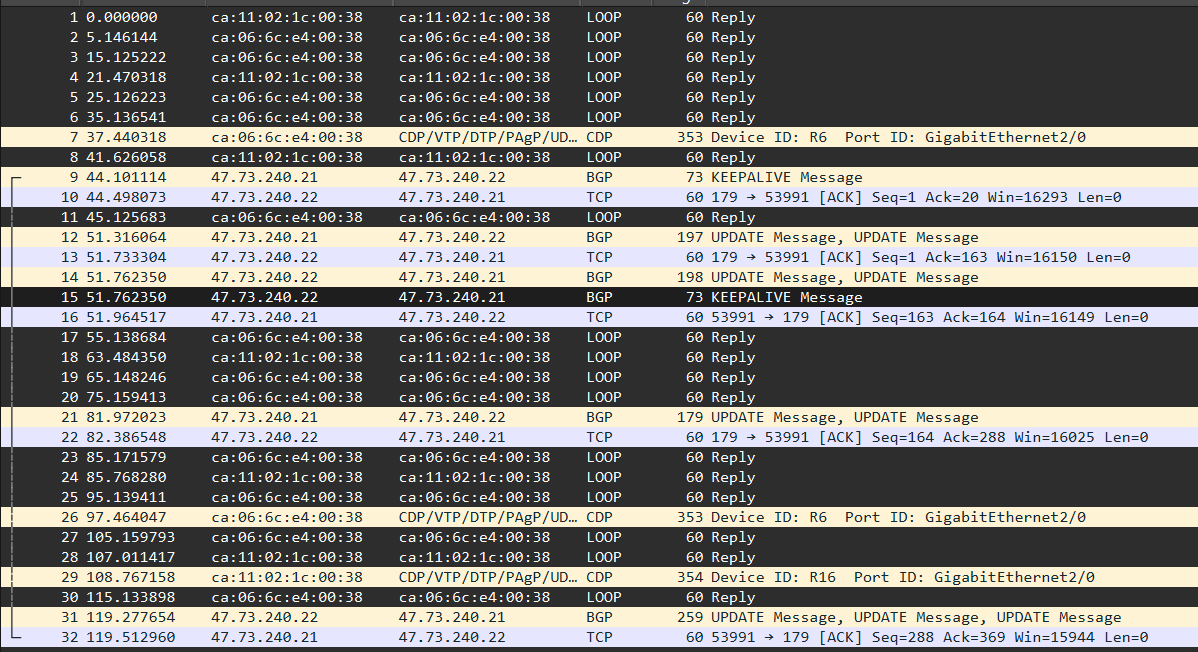
\includegraphics[width=0.80\textwidth]{imagens/Tarefa2/8.wireshark.png}
    \caption{Estabelecimento de uma sessão BGP no Wireshark}
    \label{fig:wireshark}
  \end{figure}

\end{enumerate}
\pagebreak

\section{Tarefa 3 - SCALABILITY AND ROUTING SIMPLIFICATION}
\vspace{0.2cm}

\chapter{Conclusões}
\vspace{0.2cm}


\pagebreak

\begin{thebibliography}{4} % 100 is a random guess of the total number of
  %references
  \bibitem{Slides} Documentos de apoio da UC e material fornecido pelo docente
\end{thebibliography}

\mainmatter
\end{document}